\nonstopmode
\documentclass[12pt]{report}

\title{Multilayer Perceptrons}
\author{}
\date{\today}

\usepackage[
	top=3cm,
	bottom=2cm,
	left=1.5cm,
	right=1.5cm
]{geometry}
\usepackage{amsmath}
\usepackage{amssymb}
\usepackage{amsthm}
\usepackage{amsfonts}
\usepackage{listofitems}
\usepackage{tikz}
\usepackage{pgf}
\usepackage{pgfplots}
\pgfplotsset{compat=1.18}
\usepackage[svgnames, dvipsnames, x11names]{xcolor}
\usepackage[outline]{contour} % glow around text
\usepackage[colorlinks=true, allcolors=black]{hyperref}
\contourlength{1.4pt}

\usepackage[backend=biber, style=numeric]{biblatex}

\addbibresource{./mlp.bib}

% COLORS
\colorlet{myred}{red!80!black}
\colorlet{myblue}{blue!80!black}
\colorlet{mygreen}{green!60!black}
\colorlet{myorange}{orange!70!red!60!black}
\colorlet{mydarkred}{red!30!black}
\colorlet{mydarkblue}{blue!40!black}
\colorlet{mydarkgreen}{green!30!black}
\colorlet{mydarkpurple}{violet!60!black}

\colorlet{mycaptioncol}{myblue!60}

% --------------- FONTS ---------------
% \usepackage{mathptmx}
% \usepackage{newtxtext, newtxmath}
% \usepackage{stix2}
\usepackage{mlmodern} % A better looking version of the default font
\usepackage{roboto}
\usepackage[
	font={small},
	justification=justified,
	labelfont={sf, sc, bf, color=mycaptioncol}
]{caption}
% -------------------------------------

\usetikzlibrary{arrows.meta}

% Reduce spacing for modulo
\renewcommand{\mod}{\;\text{mod}}
% Change the symbol for a QED
\renewcommand{\qedsymbol}{\blacksquare}

% Macro for a set
\newcommand{\set}[1]{\left\{ #1 \right\}}
% Macro for parentheses
\newcommand{\parens}[1]{\left( #1 \right)}
% Macro for angle brackets
\newcommand{\ang}[1]{\left\langle #1 \right\rangle}
% Macro for square brackets
\newcommand{\bracks}[1]{\left[ #1 \right]}

\tikzset{
	declare function={
		lerp(\a,\b,\t) = \a + \t * (\b - \a);
	}
}


% --------- MACROS FOR SYMBOLS ---------

% Define \bbA ... \bbZ for \mathbb
\newcommand{\bbA}{\mathbb{A}}
\newcommand{\bbB}{\mathbb{B}}
\newcommand{\bbC}{\mathbb{C}}
\newcommand{\bbD}{\mathbb{D}}
\newcommand{\bbE}{\mathbb{E}}
\newcommand{\bbF}{\mathbb{F}}
\newcommand{\bbG}{\mathbb{G}}
\newcommand{\bbH}{\mathbb{H}}
\newcommand{\bbI}{\mathbb{I}}
\newcommand{\bbJ}{\mathbb{J}}
\newcommand{\bbK}{\mathbb{K}}
\newcommand{\bbL}{\mathbb{L}}
\newcommand{\bbM}{\mathbb{M}}
\newcommand{\bbN}{\mathbb{N}}
\newcommand{\bbO}{\mathbb{O}}
\newcommand{\bbP}{\mathbb{P}}
\newcommand{\bbQ}{\mathbb{Q}}
\newcommand{\bbR}{\mathbb{R}}
\newcommand{\bbS}{\mathbb{S}}
\newcommand{\bbT}{\mathbb{T}}
\newcommand{\bbU}{\mathbb{U}}
\newcommand{\bbV}{\mathbb{V}}
\newcommand{\bbW}{\mathbb{W}}
\newcommand{\bbX}{\mathbb{X}}
\newcommand{\bbY}{\mathbb{Y}}
\newcommand{\bbZ}{\mathbb{Z}}


% Define \bfA ... \bfZ for \mathbf
\newcommand{\bfA}{\mathbf{A}}
\newcommand{\bfB}{\mathbf{B}}
\newcommand{\bfC}{\mathbf{C}}
\newcommand{\bfD}{\mathbf{D}}
\newcommand{\bfE}{\mathbf{E}}
\newcommand{\bfF}{\mathbf{F}}
\newcommand{\bfG}{\mathbf{G}}
\newcommand{\bfH}{\mathbf{H}}
\newcommand{\bfI}{\mathbf{I}}
\newcommand{\bfJ}{\mathbf{J}}
\newcommand{\bfK}{\mathbf{K}}
\newcommand{\bfL}{\mathbf{L}}
\newcommand{\bfM}{\mathbf{M}}
\newcommand{\bfN}{\mathbf{N}}
\newcommand{\bfO}{\mathbf{O}}
\newcommand{\bfP}{\mathbf{P}}
\newcommand{\bfQ}{\mathbf{Q}}
\newcommand{\bfR}{\mathbf{R}}
\newcommand{\bfS}{\mathbf{S}}
\newcommand{\bfT}{\mathbf{T}}
\newcommand{\bfU}{\mathbf{U}}
\newcommand{\bfV}{\mathbf{V}}
\newcommand{\bfW}{\mathbf{W}}
\newcommand{\bfX}{\mathbf{X}}
\newcommand{\bfY}{\mathbf{Y}}
\newcommand{\bfZ}{\mathbf{Z}}

\newcommand{\bfa}{\mathbf{a}}
\newcommand{\bfb}{\mathbf{b}}
\newcommand{\bfc}{\mathbf{c}}
\newcommand{\bfd}{\mathbf{d}}
\newcommand{\bfe}{\mathbf{e}}
\newcommand{\bff}{\mathbf{f}}
\newcommand{\bfg}{\mathbf{g}}
\newcommand{\bfh}{\mathbf{h}}
\newcommand{\bfi}{\mathbf{i}}
\newcommand{\bfj}{\mathbf{j}}
\newcommand{\bfk}{\mathbf{k}}
\newcommand{\bfl}{\mathbf{l}}
\newcommand{\bfm}{\mathbf{m}}
\newcommand{\bfn}{\mathbf{n}}
\newcommand{\bfo}{\mathbf{o}}
\newcommand{\bfp}{\mathbf{p}}
\newcommand{\bfq}{\mathbf{q}}
\newcommand{\bfr}{\mathbf{r}}
\newcommand{\bfs}{\mathbf{s}}
\newcommand{\bft}{\mathbf{t}}
\newcommand{\bfu}{\mathbf{u}}
\newcommand{\bfv}{\mathbf{v}}
\newcommand{\bfw}{\mathbf{w}}
\newcommand{\bfx}{\mathbf{x}}
\newcommand{\bfy}{\mathbf{y}}
\newcommand{\bfz}{\mathbf{z}}


% Define \calA ... \calZ for \mathcal
\newcommand{\calA}{\mathcal{A}}
\newcommand{\calB}{\mathcal{B}}
\newcommand{\calC}{\mathcal{C}}
\newcommand{\calD}{\mathcal{D}}
\newcommand{\calE}{\mathcal{E}}
\newcommand{\calF}{\mathcal{F}}
\newcommand{\calG}{\mathcal{G}}
\newcommand{\calH}{\mathcal{H}}
\newcommand{\calI}{\mathcal{I}}
\newcommand{\calJ}{\mathcal{J}}
\newcommand{\calK}{\mathcal{K}}
\newcommand{\calL}{\mathcal{L}}
\newcommand{\calM}{\mathcal{M}}
\newcommand{\calN}{\mathcal{N}}
\newcommand{\calO}{\mathcal{O}}
\newcommand{\calP}{\mathcal{P}}
\newcommand{\calQ}{\mathcal{Q}}
\newcommand{\calR}{\mathcal{R}}
\newcommand{\calS}{\mathcal{S}}
\newcommand{\calT}{\mathcal{T}}
\newcommand{\calU}{\mathcal{U}}
\newcommand{\calV}{\mathcal{V}}
\newcommand{\calW}{\mathcal{W}}
\newcommand{\calX}{\mathcal{X}}
\newcommand{\calY}{\mathcal{Y}}
\newcommand{\calZ}{\mathcal{Z}}

% --------------------------------------

\newcommand{\reffig}[1]{Figure~\ref{#1}}

% Math Operators
\DeclareMathOperator{\softmax}{softmax}
\DeclareMathOperator{\ReLU}{ReLU}
\DeclareMathOperator{\SiLU}{SiLU}
\DeclareMathOperator{\GELU}{GELU}
\DeclareMathOperator{\erf}{erf}

% =============================================
% NEURAL NETWORK DRAWING LOGIC 
% https://tikz.net/neural_networks/
% =============================================

% STYLES
\tikzset{
  >=latex, % for default LaTeX arrow head
  node/.style={thick,circle,draw=myblue,minimum size=22,inner sep=0.5,outer sep=0.6},
  node in/.style={node,green!20!black,draw=mygreen!30!black,fill=mygreen!25},
  node hidden/.style={node,blue!20!black,draw=myblue!30!black,fill=myblue!20},
  node convol/.style={node,orange!20!black,draw=myorange!30!black,fill=myorange!20},
  node out/.style={node,red!20!black,draw=myred!30!black,fill=myred!20},
  connect/.style={thick,mydarkblue}, %,line cap=round
  connect arrow/.style={-{Latex[length=4,width=3.5]},thick,mydarkblue,shorten <=0.5,shorten >=1},
  node 1/.style={node in}, % node styles, numbered for easy mapping with \nstyle
  node 2/.style={node hidden},
  node 3/.style={node out}
}
\def\nstyle{int(\lay<\Nnodlen?min(2,\lay):3)} % map layer number onto 1, 2, or 3

\pgfmathsetseed{12345}

% =============================================================
% AXES STYLE
% =============================================================

\tikzset{
	point/.style = {
		draw,
		circle,
		fill,
		inner sep = 0pt,
		minimum size = 4pt,
	},
}

\pgfplotsset{
	plane/.style={
		axis equal image,
		axis lines = middle,
		axis line style = {->},
		xlabel style = {at={(axis description cs: 1.02, 0)}, anchor = west},
		ylabel style = {at={(axis description cs: 0, 1.02)}, anchor = south},
		grid = both,
		minor tick num = 5, 
		major grid style = {thin, black!50},
		minor grid style = {very thin, black!30}
	}
}

% Arg1: General extra args for axis
% Arg2: Major grid line color + extra args
% Arg3: Minor grid line color + extra args
\NewDocumentEnvironment{plane}{O{}O{black!50}O{black!30}}{
	\begin{axis}[
		plane,
		major grid style={thin, #2},
		minor grid style={very thin, #3},
		#1
	]
}{
	\end{axis}
}

\begin{document}

\maketitle

\tableofcontents

\chapter{The Basics of Multilayer Perceptrons}

A \textbf{multilayer perceptron} (otherwise known as a \textit{neural network}) is a set of nodes called \textbf{neurons}, each containing an activation -- a number (usually) between 0 and 1 -- which designates how active that specific neuron is.

This is loosely analogous to how our brains work, where each of our neurons can fire to send an electrical signal which, somewhere down the chain, might move our arm or let us perceive the smell of some food.

The image people usually associate with neural networks is the following:

\begin{figure}[ht]
	\centering
	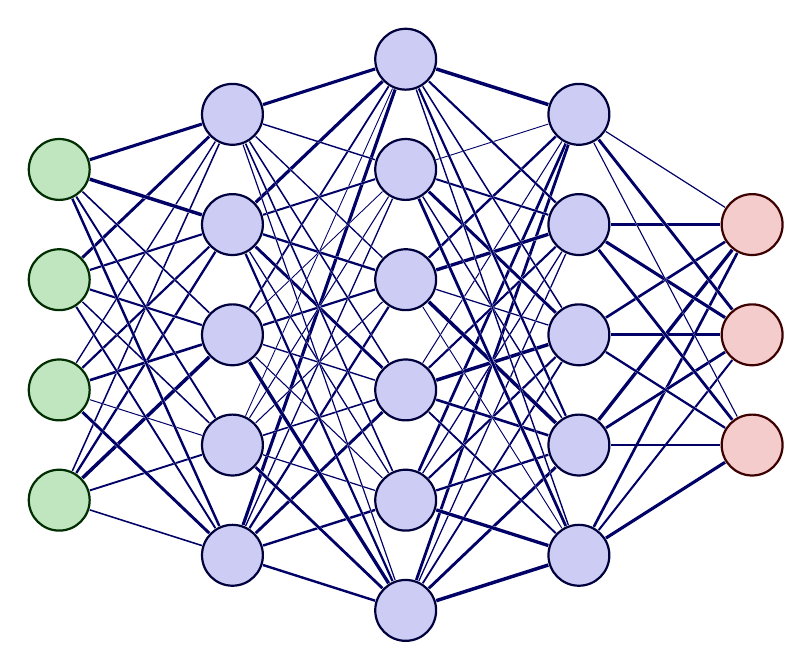
\begin{tikzpicture}[x=2.2cm,y=1.4cm]
		\readlist\Nnod{4,5,6,5,3} % array of number of nodes per layer

		% \message{^^J  Layer}
		\foreachitem \N \in \Nnod{
			\def\lay{\Ncnt} % alias of index of current layer
			\pgfmathsetmacro\prev{int(\Ncnt-1)} % number of previous layer
			% \message{\lay,}
			\foreach \i [evaluate={\y=\N/2-\i; \x=\lay; \n=\nstyle;}] in {1,...,\N}{ % loop over nodes
				  
				% NODES
				\node[node \n] (N\lay-\i) at (\x,\y) {};

				% CONNECTIONS
				\ifnum\lay>1 % connect to previous layer
					\foreach \j in {1,...,\Nnod[\prev]}{ % loop over nodes in previous layer
						\pgfmathsetmacro{\w}{0.3 + rnd}
						\draw[connect,white,line width=1.2*\w] (N\prev-\j) -- (N\lay-\i);
						\draw[connect, line width=\w] (N\prev-\j) -- (N\lay-\i);
						%\draw[connect] (N\prev-\j.0) -- (N\lay-\i.180); % connect to left
					}
				\fi % else: nothing to connect first layer
			}
		}

		% \node[above=5,align=center,mygreen!60!black] at (N1-1.90) {input\\[-0.2em]layer};
		% \node[above=2,align=center,myblue!60!black] at (N3-1.90) {hidden layers};
		% \node[above=10,align=center,myred!60!black] at (N\Nnodlen-1.90) {output\\[-0.2em]layer};
	\end{tikzpicture}
	\caption{A simple neural network.}
	\label{fig:neural-net-simple}
\end{figure}

\reffig{fig:neural-net-simple} shows the structure of a neural network. At its core, a neural network has an \textbf{input layer} (colored in green), analogous to some sensory input such as our eyes capturing the light around us, an \textbf{output layer} (colored in red), analogous to the output of our vision, which is a colored image of our environment, and then some ``hidden layers,'' which are basically the meat of the network and encode everything about how the inputs and corresponding outputs are related to one another.

\vspace{12pt}

The actual math behind these networks is surprisingly simple. We'll focus on a single connection for now:

\begin{figure}[ht]
	\centering
	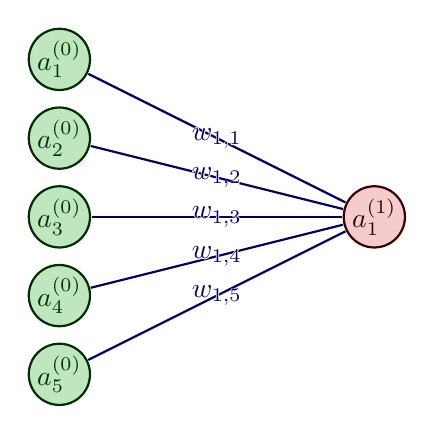
\begin{tikzpicture}
		\def\NI{5}
		\node[node 3] (second) at (2, 0) {$a_1^{(1)}$};
		\foreach \i [evaluate={\y=(\NI + 1) / 2 - \i; \index = int(\i)}] in {1,...,\NI} {
			\node[node 1] (NI-\i) at (-2, \y) {$a_{\index}^{(0)}$};
			\draw[connect] (NI-\i) -- (second) node[midway] {\contour{white}{$w_{1,\index}$}};
		}
	\end{tikzpicture}
	\caption{The activation of two neurons and the weight between them.}
	\label{fig:neuron-activation-example}
\end{figure}

Let's decypher these symbols one-by-one:
\begin{itemize}
	\item ${\color{mydarkgreen} a_n^{(0)}}$: The activations of the nodes within the first layer.
	\item ${\color{mydarkblue} w_{1,n}}$: The \textbf{weights} of each of the connections. Essentially, this encodes how strongly connected the neurons are (so how much they influence each-other).
	\item ${\color{mydarkred} a_1^{(1)}}$: The output activation.
\end{itemize}

In order to determine the output activation $a_1^{(1)}$ from the input activations $a_i^{(0)}$, we simply take a weighted sum whose weights are the coefficients $w_{1,i}$; that is,
\[
	{\color{mydarkred} a_1^{(1)}} = {\color{mydarkblue} w_{1,1}}{\color{mydarkgreen} a_1^{(0)}} + {\color{mydarkblue} w_{1,2}}{\color{mydarkgreen} a_2^{(0)}} + \cdots + {\color{mydarkblue} w_{1,5}}{\color{mydarkgreen} a_5^{(0)}}
\]

Usually we also add in what's called a \textbf{bias} term, which is just a value that we add to this sum. We can interpret the bias as the ``sensitivity'' of the neuron. That means that the whole expression in the general case (so, for $n$ neurons in the input layer) is
\[
	{\color{mydarkred} a_1^{(1)}} = {\color{mydarkpurple}b_1^{(0)}} + \sum_{i=1}^{n}{\color{mydarkblue} w_{1,i}}{\color{mydarkgreen} a_i^{(0)}}
\]

There's only one issue: Remember we said that the activations must be between 0 and 1, but with a weighted sum like this, we can essentially get any number. What we need now is some kind of way to squish this value into the range $[0,1]$. The most common function for this purpose is the \textbf{sigmoid} function:
\[
	{\color{mydarkred}\sigma({\color{mydarkblue}x})} = \frac{1}{1 + e^{-{\color{mydarkblue}x}}}
\]

The graph of this function is shown below:

\begin{figure}[ht]
	\centering
	\begin{tikzpicture}
		\begin{plane}[
			tick label style = {font = \small},
			xmin = -4,
			xmax = 4,
			ymin = -3,
			ymax = 3
		]
			\addplot[mydarkblue, smooth, ultra thick] {1 / (1 + exp(-x))};
		\end{plane}
	\end{tikzpicture}
	\caption{The graph of $\sigma(x)$.}
	\label{fig:sigmoid-graph}
\end{figure}

\newpage

From \reffig{fig:sigmoid-graph}, we can see how the function approaches 0 when $x$ is negative, and approaches 1 when $x$ is positive. This is exactly what we needed! Putting all of this together, we have the following expression for ${\color{mydarkred}a_1^{(1)}}$:
\[
	{\color{mydarkred}a_1^{(1)}} = {\color{mydarkred}\sigma}{\color{mydarkred}\Bigg(}{\color{mydarkpurple}b_1^{(0)}}{\color{black} + \sum_{i=1}^{n}}{\color{mydarkblue}w_{1,i}}{\color{mydarkgreen}a_i^{(0)}}{\color{mydarkred}\Bigg)}
\]

Remember, this is just for the activation of a \textit{single} neuron, so for a whole layer, we need to do this many times. There is a way we can simplify this, but we'll need to consider the more general case in order to do so.

\begin{figure}[ht]
	\centering
	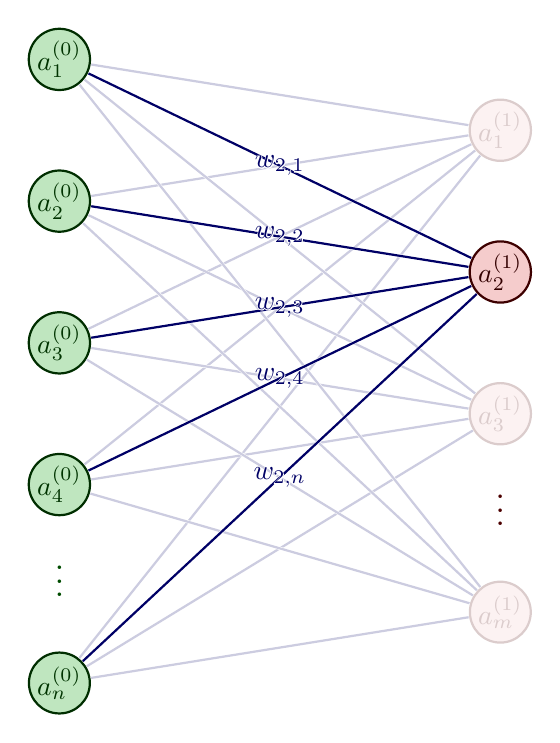
\begin{tikzpicture}[x=1.4cm, y = 1.8cm]
		\def\NI{5}
		\def\NO{4}
		\def\NodeFocused{2}
		\def\yshift{0.4}

		% Input Layer
		\foreach \i [evaluate={\c=int(\i==\NI); \y=\NI / 2 - \i - \c*\yshift; \index=(\i < \NI ? int(\i) : "n");}] in {1,...,\NI}{
			\node[node in] (NI-\i) at (-2,\y) {$a_{\index}^{(0)}$};
		}

		\foreach \i [evaluate={\c=int(\i==\NO); \y=\NO / 2 - \i - \c * \yshift; \indexout = (\i < \NO ? int(\i) : "m");}] in {1,...,\NO}{
			\ifnum\i=\NodeFocused
				% skip for now
			\else
				\node[node, color=mydarkred!20, fill=myred!5] (NO-\i) at (2,\y) {$a_{\indexout}^{(1)}$};
				\foreach \j [evaluate={\indexin=int(\j);}] in {1,...,\NI}{
					\draw[connect, white, line width = 1.2] (NI-\j) -- (NO-\i);
					\draw[connect, mydarkblue!20] (NI-\j) -- (NO-\i);
				}
			\fi
		}

		\pgfmathsetmacro\yfocused{\NO/2-\NodeFocused-int(\NodeFocused==\NO) * \yshift}
		\pgfmathsetmacro\indexout{(\NodeFocused < \NO ? int(\NodeFocused) : "m")}
		
		% Draw the focused node after everything else
		\node[node out] (NO-\NodeFocused) at (2,\yfocused) {$a_{\indexout}^{(1)}$};

		\foreach \j [evaluate={\indexin=(\j < \NI ? int(\j) : "n");}] in {1,...,\NI}{
			\draw[connect, white, line width = 1.2] (NI-\j) -- (NO-\NodeFocused);
			\draw[connect] (NI-\j) -- (NO-\NodeFocused) node[midway] {\contour{white}{$w_{\indexout,\indexin}$}};
		}

		\path[color=mydarkgreen] (NI-\NI) --++ (0,0.95+\yshift) node[midway,scale=1.2] {$\vdots$};
	  \path[color=mydarkred] (NO-\NO) --++ (0,0.95+\yshift) node[midway,scale=1.2] {$\vdots$};
	\end{tikzpicture}
	\caption{The general case of the connections between two layers.}
	\label{fig:general-connection-case}
\end{figure}

The key insight here is that we can simplify this process immensely with the tools of linear algebra. In particular, we can group all the activations in the first layer (layer 0) into a column vector:
\[
	{\color{mydarkgreen} \bfa^{(0)}} = {\color{mydarkgreen}\begin{bmatrix}
			a_1^{(0)}\\
			a_2^{(0)}\\
			\vdots\\
			a_n^{(0)}
	\end{bmatrix}}
\]

\noindent
We can do the same thing for the output activations:
\[
	{\color{mydarkred} \bfa^{(1)}} = {\color{mydarkred}\begin{bmatrix}
			a_1^{(1)}\\
			a_2^{(1)}\\
			\vdots\\
			a_m^{(1)}
		\end{bmatrix}}
\]

\noindent
Similarly, we can group the biases up into a vector as well:
\[
	{\color{mydarkpurple} \bfb^{(0)}} = {\color{mydarkpurple}\begin{bmatrix}
			b_1^{(0)}\\
			b_2^{(0)}\\
			\vdots\\
			b_m^{(0)}
		\end{bmatrix}}
\]

\noindent
Finally, the weights simply become a matrix which we multiply with ${\color{mydarkgreen}\bfa^{(0)}}$:

\[
	{\color{mydarkblue} \bfW^{(0)}} = {\color{mydarkblue}\begin{bmatrix}
			w_{1,1} && w_{1,2} && w_{1,3} && \cdots && w_{1,n}\\
			w_{2,1} && w_{2,2} && w_{2,3} && \cdots && w_{2,n}\\
			w_{3,1} && w_{3,2} && w_{3,3} && \cdots && w_{3,n}\\
			\vdots  && \vdots  && \vdots  && \ddots && \vdots \\
			w_{m,1} && w_{m,2} && w_{m,3} && \cdots && w_{m,n}
		\end{bmatrix}}
\]

\noindent
Now, if we imply that the function $\sigma(x)$ applies component-wise to vectors and matrices, we get the following incredibly neat formula for the activations in layer $L + 1$ given those in layer $L$:
\[
	{\color{mydarkred}\bfa^{(L+1)}} = {\color{mydarkred}\sigma}{\color{mydarkred}\big(}{\color{mydarkpurple}\bfb^{(L)}} + {\color{mydarkblue}\bfW^{(L)}}{\color{mydarkgreen}\bfa^{(L)}}{\color{mydarkred}\big)}
\]

\newpage

\addcontentsline{section}{toc}{Other Activation Functions}
\section*{Other Activation Functions}

The sigmoid is not the only function we can use to remap our values. In fact, there are infinitely many functions we can use. Another common choice is the $\tanh$ function (which remaps values between $-1$ and 1). Beyond that, we sometimes don't want to remap between finite values at all. This is why other (arguably more common) activation functions include the $\ReLU$, $\SiLU$, and, more recently, $\GELU$ functions.

\begin{figure}[ht]
	\centering
	\begin{tikzpicture}[
		declare function={
			sigmoid(\x) = 1 / (1 + exp(-\x));
			relu(\x) = max(\x, 0);
			silu(\x) = \x * sigmoid(\x);
			gelu(\x) = 0.5 * \x * (1 + tanh(sqrt(2 / pi) * (\x + 0.044715 * \x^3)));
		},
		scale=1.25
	]
		\begin{plane}[
			xmin = -3,
			xmax = 3,
			ymin = -3,
			ymax = 3,
			legend style = {font=\scriptsize},
			legend cell align=left,
			legend pos = north west,
			tick label style = {font = \small},
		]
			\addplot[very thick, smooth, black] {tanh(x)};
			\addlegendentry{$\tanh(x)$}
			\addplot[very thick, smooth, LimeGreen] {silu(x)};
			\addlegendentry{$\SiLU(x)$}
			\addplot[very thick, smooth, TealBlue] {gelu(x)};
			\addlegendentry{$\GELU(x)$}
			\addplot[very thick, smooth, samples=200, OrangeRed] {relu(x)};
			\addlegendentry{$\ReLU(x)$}
		\end{plane}
	\end{tikzpicture}
	\caption{The graphs of the different activation functions.}
	\label{fig:activation-functions}
\end{figure}

$\ReLU$ is very common because it's very strict for model behavior; the activation simply gets clamped to zero if it's negative. The expressions for these functions are the following:
\begin{align*}
	\ReLU(x) &= \max(x, 0)\\
	\SiLU(x) &= x \sigma(x)\\
	\GELU(x) &\approx 0.5x\parens{1 + \tanh\parens{\sqrt{\frac{2}{\pi}}\parens{x + 0.044715x^3}}}\text{\cite{hendrycks2023gelu}}
\end{align*}

The expression for $\GELU$ is simply an approximation because it is actually derived from the cumulative distribution function of the normal distribution, which has no elementary form. In fact, the \textit{true} expression defining $\GELU(x)$ is 
\[
	\GELU(x) = x\Phi(x) = x\frac{1}{2}\bracks{1 + \erf\parens{\frac{x}{\sqrt{2}}}},
\]
where 
\[
	\erf(x) = \int_0^x e^{-s^2}ds
\]
is the error function.

% \begin{figure}[ht]
% 	\centering
% 	% NEURAL NETWORK activation
% 	% https://www.youtube.com/watch?v=aircAruvnKk&list=PLZHQObOWTQDNU6R1_67000Dx_ZCJB-3pi&index=1
% 	\begin{tikzpicture}[x=2.7cm,y=1.6cm]
% 	  \message{^^JNeural network activation}
% 	  \def\NI{5} % number of nodes in input layers
% 	  \def\NO{4} % number of nodes in output layers
% 	  \def\yshift{0.4} % shift last node for dots
	  
% 	  % INPUT LAYER
% 	  \foreach \i [evaluate={\c=int(\i==\NI); \y=\NI/2-\i-\c*\yshift; \index=(\i<\NI?int(\i):"n");}]
% 	              in {1,...,\NI}{ % loop over nodes
% 	    \node[node in,outer sep=0.6] (NI-\i) at (0,\y) {$a_{\index}^{(0)}$};
% 	  }
	  
% 	  % OUTPUT LAYER
% 	  \foreach \i [evaluate={\c=int(\i==\NO); \y=\NO/2-\i-\c*\yshift; \index=(\i<\NO?int(\i):"m");}]
% 	    in {\NO,...,1}{ % loop over nodes
% 	    \ifnum\i=1 % high-lighted node
% 	      \node[node hidden]
% 	        (NO-\i) at (1,\y) {$a_{\index}^{(1)}$};
% 	      \foreach \j [evaluate={\index=(\j<\NI?int(\j):"n");}] in {1,...,\NI}{ % loop over nodes in previous layer
% 	        \draw[connect,white,line width=1.2] (NI-\j) -- (NO-\i);
% 	        \draw[connect] (NI-\j) -- (NO-\i)
% 	          node[pos=0.50] {\contour{white}{$w_{1,\index}$}};
% 	      }
% 	    \else % other light-colored nodes
% 	      \node[node,blue!20!black!80,draw=myblue!20,fill=myblue!5]
% 	        (NO-\i) at (1,\y) {$a_{\index}^{(1)}$};
% 	      \foreach \j in {1,...,\NI}{ % loop over nodes in previous layer
% 	        %\draw[connect,white,line width=1.2] (NI-\j) -- (NO-\i);
% 	        \draw[connect,myblue!20] (NI-\j) -- (NO-\i);
% 	      }
% 	    \fi
% 	  }
	  
% 	  % DOTS
% 	  \path (NI-\NI) --++ (0,1+\yshift) node[midway,scale=1.2] {$\vdots$};
% 	  \path (NO-\NO) --++ (0,1+\yshift) node[midway,scale=1.2] {$\vdots$};
	  
% 	  % EQUATIONS
% 	  \def\agr#1{{\color{mydarkgreen}a_{#1}^{(0)}}} % green a_i^j
% 	  \node[below=16,right=11,mydarkblue,scale=0.95] at (NO-1)
% 	    {$\begin{aligned} %\underset{\text{bias}}{b_1}
% 	       &= \color{mydarkred}\sigma\left( \color{black}
% 	            w_{1,1}\agr{1} + w_{1,2}\agr{2} + \ldots + w_{1,n}\agr{n} + b_1^{(0)}
% 	          \color{mydarkred}\right)\\
% 	       &= \color{mydarkred}\sigma\left( \color{black}
% 	            \sum_{i=1}^{n} w_{1,i}\agr{i} + b_1^{(0)}
% 	           \color{mydarkred}\right)
% 	     \end{aligned}$};
% 	  \node[right,scale=0.9] at (1.3,-1.3)
% 	    {$\begin{aligned}
% 	      {\color{mydarkblue}
% 	      \begin{pmatrix}
% 	        a_{1}^{(1)} \\[0.3em]
% 	        a_{2}^{(1)} \\
% 	        \vdots \\
% 	        a_{m}^{(1)}
% 	      \end{pmatrix}}
% 	      &=
% 	      \color{mydarkred}\sigma\left[ \color{black}
% 	      \begin{pmatrix}
% 	        w_{1,1} & w_{1,2} & \ldots & w_{1,n} \\
% 	        w_{2,1} & w_{2,2} & \ldots & w_{2,n} \\
% 	        \vdots  & \vdots  & \ddots & \vdots  \\
% 	        w_{m,1} & w_{m,2} & \ldots & w_{m,n}
% 	      \end{pmatrix}
% 	      {\color{mydarkgreen}
% 	      \begin{pmatrix}
% 	        a_{1}^{(0)} \\[0.3em]
% 	        a_{2}^{(0)} \\
% 	        \vdots \\
% 	        a_{n}^{(0)}
% 	      \end{pmatrix}}
% 	      +
% 	      \begin{pmatrix}
% 	        b_{1}^{(0)} \\[0.3em]
% 	        b_{2}^{(0)} \\
% 	        \vdots \\
% 	        b_{m}^{(0)}
% 	      \end{pmatrix}
% 	      \color{mydarkred}\right]\\[0.5em]
% 	      {\color{mydarkblue}\mathbf{a}^{(1)}} % vector (bold)
% 	      &= \color{mydarkred}\sigma\left( \color{black}
% 	           \mathbf{W}^{(0)} {\color{mydarkgreen}\mathbf{a}^{(0)}}+\mathbf{b}^{(0)}
% 	         \color{mydarkred}\right)
% 	    \end{aligned}$};
	  
% 	\end{tikzpicture}
% 	\caption{The calculation for the activation $a_1^{(1)}$.}
% 	\label{fig:neural-net-focus-node}
% \end{figure}

\printbibliography

\end{document}